\subsection[二次曲面]{Conic Section/Curve \& Quadric Surface}

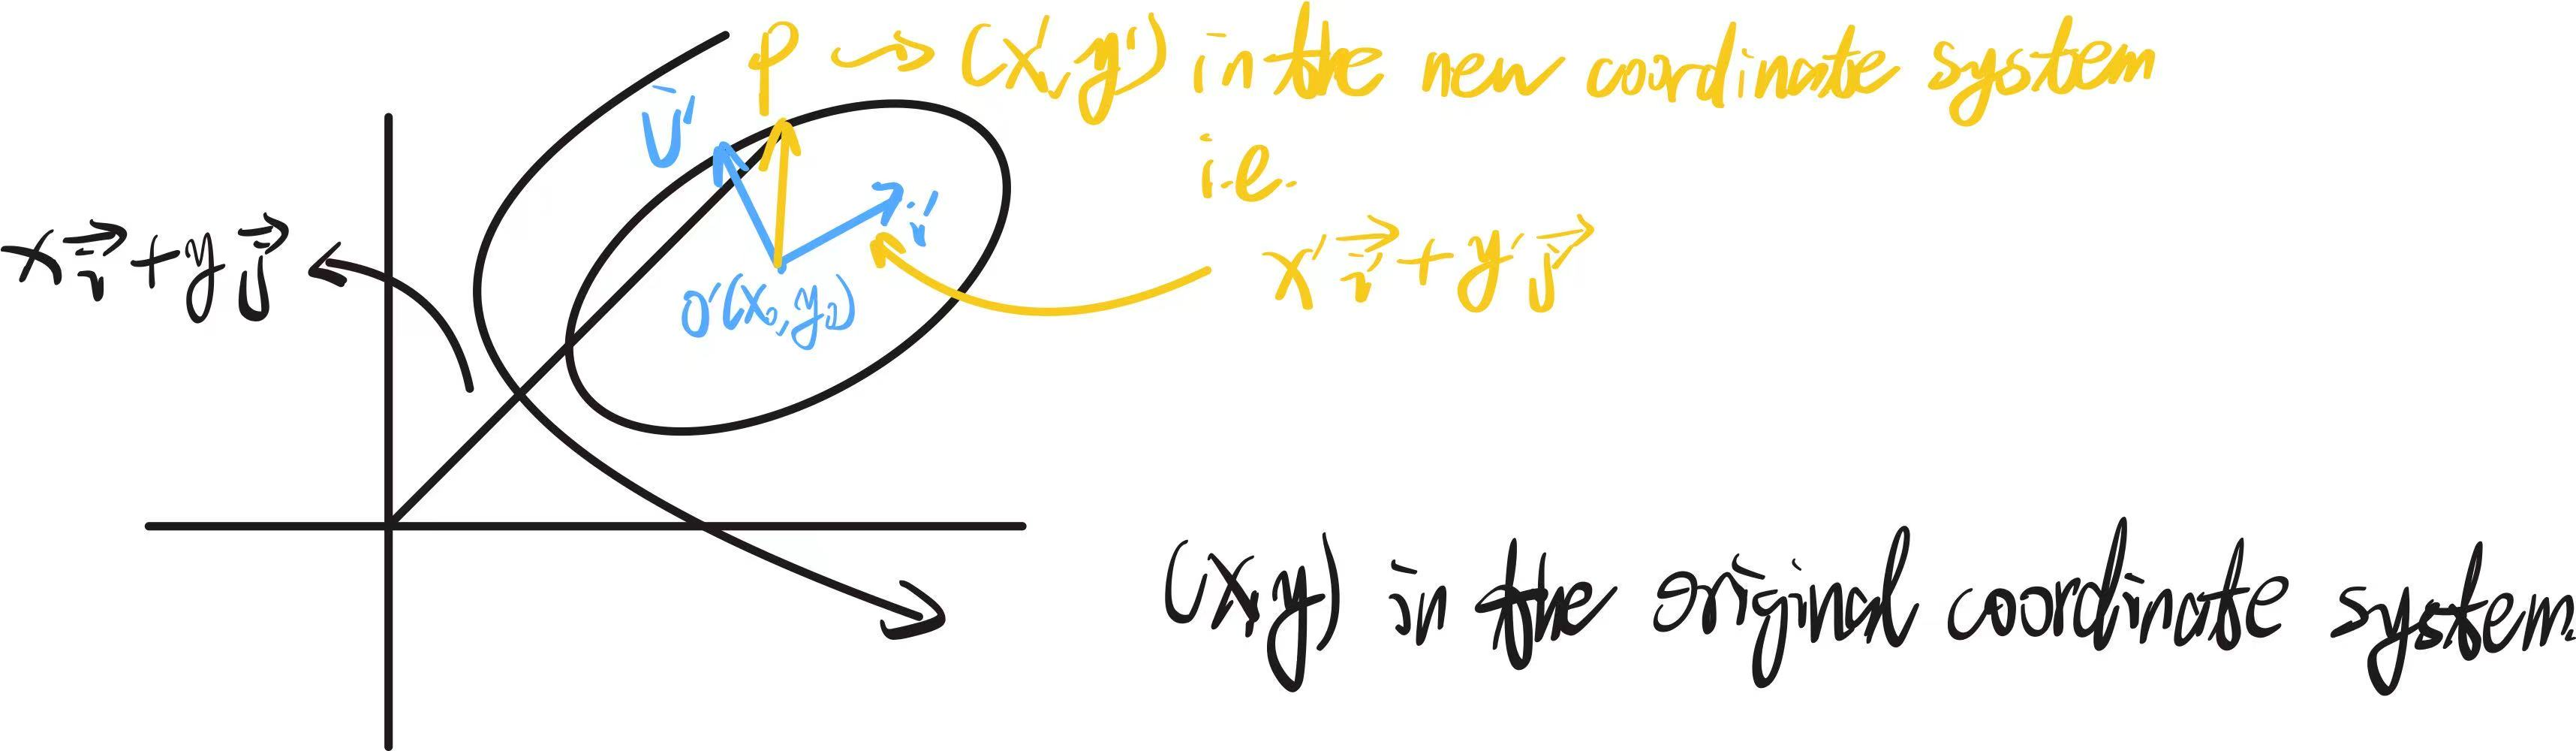
\includegraphics[height=3cm]{chapters/08/CSCQS01}

$\implies\begin{pmatrix}\overrightarrow{i}&\overrightarrow{j}\end{pmatrix}\begin{pmatrix}x\\y\end{pmatrix}=\overrightarrow{OP}=\underset{=\begin{pmatrix}\overrightarrow{i}&\overrightarrow{j}\end{pmatrix}\begin{pmatrix}x_0\\y_0\end{pmatrix}}{\overrightarrow{OO'}}+\underset{=\underset{=\begin{pmatrix}\overrightarrow{i}&\overrightarrow{j}\end{pmatrix}\begin{pmatrix}x'\\y'\end{pmatrix}}{\begin{pmatrix}\overrightarrow{i'}&\overrightarrow{j'}\end{pmatrix}}\begin{pmatrix}x'\\y'\end{pmatrix}}{\overrightarrow{O'P}}$

$\implies\begin{pmatrix}x\\y\end{pmatrix}=P\begin{pmatrix}x'\\y'\end{pmatrix}+\begin{pmatrix}x_0\\y_0\end{pmatrix}$ coordinate transformation

\subsubsection*{Quadric in $\mathbb{R}^n$}

\begin{align*}
    f\left(x_1,\dots,x_n\right) & =\sum_{i,j=1}^{n}x_iA_{ij}x_j+\sum_{i=1}^n b_i x_i+C\text{, where }A=A^T \\
                                & =X^TAX+b^TX+C\text{, where }X=\begin{pmatrix}
                                                                    x_1 \\\vdots\\x_n
                                                                \end{pmatrix}
\end{align*}

Question: Can we find coordinate transformation $x=Py$ where $P\in O(n)$ to simplify the expression:
$$y^TP^TAPy+b^TPy+C$$

\begin{enumerate}
    \item Take $P$ s.t. $$P^TAP=\begin{pmatrix}
                  \lambda_1 &        &               &                  &        &                   &   &        &   \\
                            & \ddots &               &                  &        &                   &   &        &   \\
                            &        & \lambda_{r_+} &                  &        &                   &   &        &   \\
                            &        &               & -\lambda_{r_++1} &        &                   &   &        &   \\
                            &        &               &                  & \ddots &                   &   &        &   \\
                            &        &               &                  &        & \lambda_{r_++r_-} &   &        &   \\
                            &        &               &                  &        &                   & 0 &        &   \\
                            &        &               &                  &        &                   &   & \ddots &   \\
                            &        &               &                  &        &                   &   &        & 0
              \end{pmatrix}$$
    \item $y=z+\left(\vdots\right)$
    \item \allbold{$\lambda_1z_1^2+\dots+\lambda_{r_+}z_{r_+}^2-\left(\lambda_{r_++1}z_{r_++1}^2+\dots\right)$}
\end{enumerate}